\documentclass[a4paper,12pt]{scrreprt}

\usepackage{ucs}				%auch UTF8 package, gleich wie utf8x{inputenc}
%\usepackage[utf8x]{inputenc}	%damit man UTF8 benutzt
\usepackage[ngerman]{babel}		%für ä,ö,ü usw.
\usepackage{graphicx} 			%zum Bilder einfügen
%\usepackage[T1]{fontenc}		%andere Schriftart
\usepackage{amssymb}			%für Symbol

%SCR PAGESTYLE

%\usepackage{scrlayer-scrpage}			%Package laden
%\pagestyle{scrheadings}
%\clearpairofpagestyles			%lösche alle Kopf und Fußzeilen
%\automark{chapter}				%Autoerkenneung Chapter
%\ohead{Projektarbeit}
%\cfoot{\pagemark}% Seitenzahl
%\renewcommand{\chaptermark}[1]{\markright{\ #1}} %löscht die Nummerierung von Chapter
%\ihead{\textbf{\rightchapter}}

\renewcommand{\chapterpagestyle}{fancy} 	%Kopfzeile auch auf Chapter-Seiten

%FANCY PAGESTYLE

\usepackage{fancyhdr}
\pagestyle{fancy}

\lhead{Tommy Köhler}
\chead{}
\rhead{Projektarbeit}

\lfoot{}
\cfoot{\thepage}
\rfoot{}

\renewcommand{\headrulewidth}{0.4pt}
\renewcommand{\footrulewidth}{0pt}

\begin{document}

\thispagestyle{empty}

\begin{center}
	{\LARGE \textbf{Thema der Projektarbeit}}\\
	\vspace{2.0cm}				%Abstand zur nächsten Zeile
	{\Huge \textbf{Projektarbeit}}\\
	\vspace{1.0cm}
	vorgelegt am \today\\
	\vspace{2.0cm}
	
\begin{tabular}{rl}
	von:				& Tommy Köhler\\
						& Mahlen 27\\
						& 06172 Zeitz\\
						& \\
	Matrikelnummer: 	& ..........\\
						& \\
	DHGE Campus:		& Gera\\
						& \\
	Studienbereich:		& Technik\\
						& \\
	Studiengang:		& Technische Informatik\\
						& \\
	Kurs:				& Kurs\\
						& \\
						& \\
	Ausbildungsstätte:	& Indu-Sol GmbH\\
						& Blumenstraße 3\\
						& 04626 Schmölln\\
						& \\
	Betreuer:			& ............ \\
						& ............ \\
						
						
\end{tabular}
\end{center}

\tableofcontents

\chapter{Einleitung}
\label{scr:Einleitung}
Lorem ipsum dolor sit amet, consetetur sadipscing elitr, sed diam nonumy eirmod tempor invidunt ut labore et dolore magna aliquyam erat, sed diam voluptua. At vero eos et accusam et justo duo dolores et ea rebum. Stet clita kasd gubergren, no sea takimata sanctus est Lorem ipsum dolor sit amet. Lorem ipsum dolor sit amet, consetetur sadipscing elitr, sed diam nonumy eirmod tempor invidunt ut labore et dolore magna aliquyam erat, sed diam voluptua. At vero eos et accusam et justo duo dolores et ea rebum. Stet clita kasd gubergren, no sea takimata sanctus est Lorem ipsum dolor sit amet. Lorem ipsum dolor sit amet, consetetur sadipscing elitr, sed diam nonumy eirmod tempor invidunt ut labore et dolore magna aliquyam erat, sed diam voluptua. At vero eos et accusam et justo duo dolores et ea rebum. Stet clita kasd gubergren, no sea takimata sanctus est Lorem ipsum dolor sit amet.



Duis autem vel eum iriure dolor in hendrerit in vulputate velit esse molestie consequat, vel illum dolore eu feugiat nulla facilisis at vero eros et accumsan et iusto odio dignissim qui blandit praesent luptatum zzril delenit augue duis dolore te feugait nulla facilisi. Lorem ipsum dolor sit amet, consectetuer adipiscing Lorem ipsum dolor sit amet, consetetur sadipscing elitr, sed diam nonumy eirmod tempor invidunt ut labore et dolore magna aliquyam erat, sed diam voluptua. At vero eos et accusam et justo duo dolores et ea rebum. Stet clita kasd gubergren, no sea takimata sanctus est Lorem ipsum dolor sit amet. Lorem ipsum dolor sit amet, consetetur sadipscing elitr, sed diam nonumy eirmod tempor invidunt ut labore et dolore magna aliquyam.

\chapter{Hauptteil}
\label{sec:Hauptteil}

\section{Ipsum dolor}
Lorem ipsum dolor sit amet, consetetur sadipscing elitr, sed diam nonumy eirmod tempor invidunt ut labore et dolore magna aliquyam erat, sed diam voluptua. At vero eos et accusam et justo duo dolores et ea rebum. Stet clita kasd gubergren, no sea takimata sanctus est Lorem ipsum dolor sit amet. Lorem ipsum dolor sit amet, consetetur sadipscing elitr, sed diam nonumy eirmod tempor invidunt ut labore et dolore magna aliquyam erat, sed diam voluptua. At vero eos et accusam et justo duo dolores et ea rebum. Stet clita kasd gubergren, no sea takimata sanctus est Lorem ipsum dolor sit amet.

\section{consetetur sadipscing}
Lorem ipsum dolor sit amet, consetetur sadipscing elitr, sed diam nonumy eirmod tempor invidunt ut labore et dolore magna aliquyam erat, sed diam voluptua. At vero eos et accusam et justo duo dolores et ea rebum. Stet clita kasd gubergren, no sea takimata sanctus est Lorem ipsum dolor sit amet. Lorem ipsum dolor sit amet, consetetur sadipscing elitr, sed diam nonumy eirmod tempor invidunt ut labore et dolore magna aliquyam erat, sed diam voluptua. At vero eos et accusam et justo duo dolores et ea rebum. Stet clita kasd gubergren, no sea takimata sanctus est Lorem ipsum dolor sit amet. Lorem ipsum dolor sit amet, consetetur sadipscing elitr, sed diam nonumy eirmod tempor invidunt ut labore et dolore magna aliquyam erat, sed diam voluptua. At vero eos et accusam et justo duo dolores et ea rebum. Stet clita kasd gubergren, no sea takimata sanctus est Lorem ipsum dolor sit amet.

\newpage

\subsection{et accusam}
Lorem ipsum dolor sit amet, consetetur sadipscing elitr, sed diam nonumy eirmod tempor invidunt ut labore et dolore magna aliquyam erat, sed diam voluptua. At vero eos et accusam et justo duo dolores et ea rebum. Stet clita kasd gubergren, no sea takimata sanctus est Lorem ipsum dolor sit amet. Lorem ipsum dolor sit amet, consetetur sadipscing elitr, sed diam nonumy eirmod tempor invidunt ut labore et dolore magna aliquyam
 Lorem ipsum dolor sit amet, consetetur sadipscing elitr, sed diam nonumy eirmod tempor invidunt ut labore et dolore magna aliquyam erat, sed diam voluptua. At vero eos et accusam et justo duo dolores et ea rebum. Stet clita kasd gubergren, no sea takimata sanctus est Lorem ipsum dolor sit amet. Lorem ipsum dolor sit amet, consetetur sadipscing elitr, sed diam nonumy eirmod tempor invidunt ut labore et dolore magna aliquyam erat, sed diam voluptua. At vero eos et accusam et justo duo dolores et ea rebum. Stet clita kasd gubergren, no sea takimata sanctus est Lorem ipsum dolor sit amet. Lorem ipsum dolor sit amet, consetetur sadipscing elitr, sed diam nonumy eirmod tempor invidunt ut labore et dolore magna aliquyam erat, sed diam voluptua. At vero eos et accusam et justo duo dolores et ea rebum. Stet clita kasd gubergren, no sea takimata sanctus est Lorem ipsum dolor sit amet.   

Duis autem vel eum iriure dolor in hendrerit in vulputate velit esse molestie consequat, vel illum dolore eu feugiat nulla facilisis at vero eros et accumsan et iusto



\chapter{Anhang}
\label{scr:Anhang}
Möglicher Anhang...Bilder usw.

Hierzu zB. JabRef nutzen!



Nachfolgend mal noch ein komplettes PDF eingebunden:

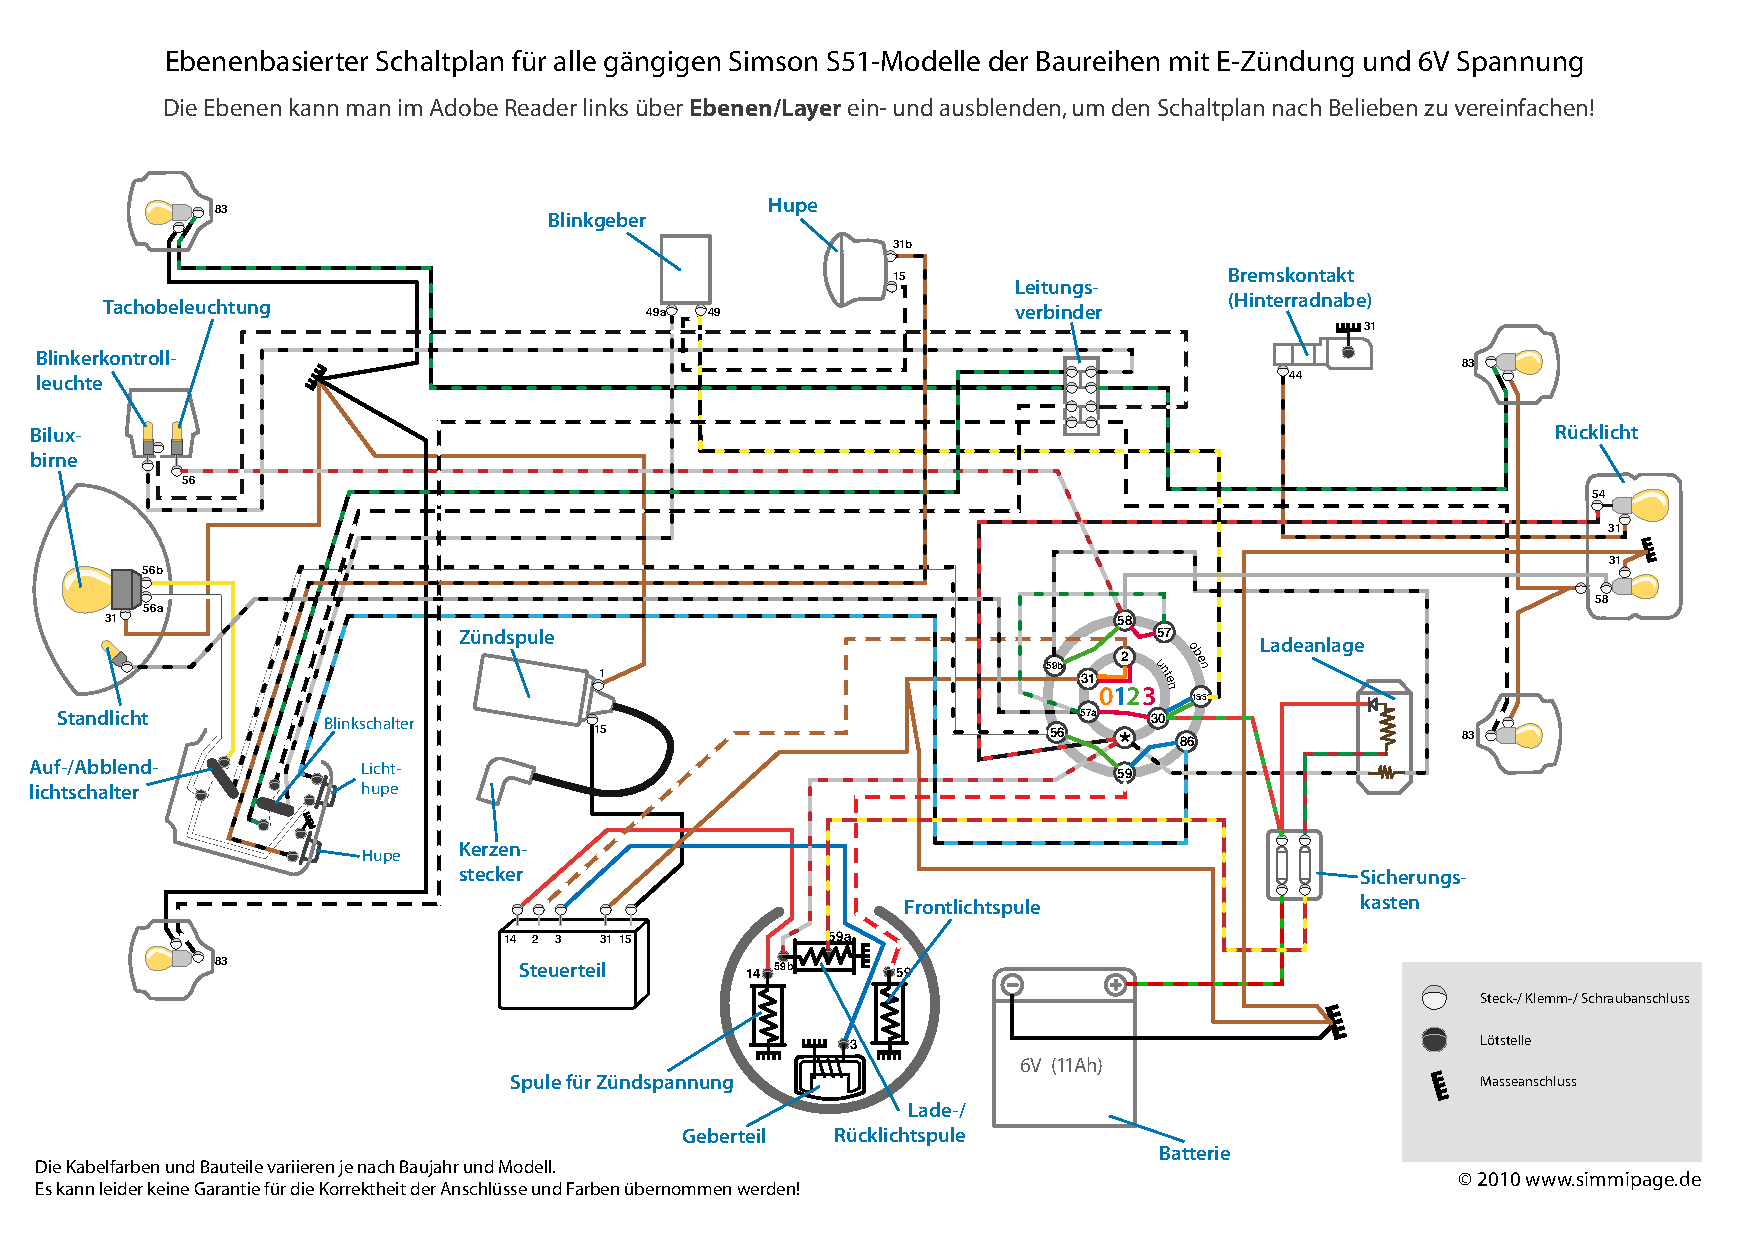
\includepdf[pages=-]{Elektronikzundung_Schaltplan}

\end{document}